\documentclass[border=4pt]{standalone}
\usepackage{tikz}
\usepackage{pgfplots}
\pgfplotsset{compat=1.18}
\usetikzlibrary{positioning, calc}
\begin{document}
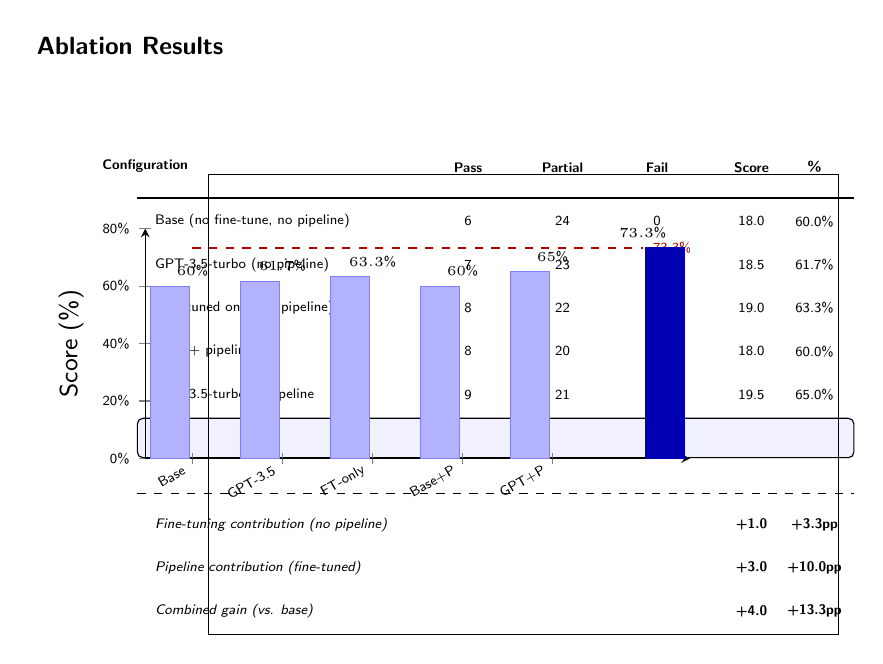
\begin{tikzpicture}
% ==================== TABLE SECTION ====================
% Recreate the ablation table as structured nodes

% Header row
\foreach \x/\txt in {0/Configuration, 4.1/Pass, 5.3/Partial, 6.5/Fail, 7.7/Score, 8.5/\%}
  \node[font=\tiny\sffamily\bfseries, anchor=south, minimum height=1.0em]
    at (\x, 3.5) {\txt};

% Horizontal line below header
\draw[thick] (-0.1,3.3) -- (9.0,3.3);

% Data rows (y position from 3.0 down to -1.0)
\newcommand{\datarow}[7]{%
  \pgfmathparse{3.0 - (#1 - 1) * 0.55}%
  \let\y\pgfmathresult
  \node[font=\tiny\sffamily, anchor=west] at (0,\y) {#2};
  \node[font=\tiny\sffamily, anchor=center] at (4.1,\y) {#3};
  \node[font=\tiny\sffamily, anchor=center] at (5.3,\y) {#4};
  \node[font=\tiny\sffamily, anchor=center] at (6.5,\y) {#5};
  \node[font=\tiny\sffamily, anchor=center] at (7.7,\y) {#6};
  \node[font=\tiny\sffamily, anchor=center] at (8.5,\y) {#7};
}

\datarow{1}{Base (no fine-tune, no pipeline)}{6}{24}{0}{18.0}{60.0\%}
\datarow{2}{GPT-3.5-turbo (no pipeline)}{7}{23}{0}{18.5}{61.7\%}
\datarow{3}{Fine-tuned only (no pipeline)}{8}{22}{0}{19.0}{63.3\%}
\datarow{4}{Base + pipeline}{8}{20}{2}{18.0}{60.0\%}
\datarow{5}{GPT-3.5-turbo + pipeline}{9}{21}{0}{19.5}{65.0\%}
\datarow{6}{ThreadLearn + pipeline}{14}{16}{0}{22.0}{73.3\%}

% Highlight ThreadLearn row
\draw[fill=blue!6, rounded corners=2pt] (-0.1,{3.0 - 5*0.55 - 0.25}) rectangle (9.0,{3.0 - 5*0.55 + 0.25});

% Summary rows
\draw[thin, dashed] (-0.1,{3.0 - 6*0.55 - 0.15}) -- (9.0,{3.0 - 6*0.55 - 0.15});
% Fine-tuning contribution
\node[font=\tiny\sffamily\itshape, anchor=west] at (0,{3.0 - 7*0.55}) {Fine-tuning contribution (no pipeline)};
\node[font=\tiny\sffamily\bfseries, anchor=center] at (7.7,{3.0 - 7*0.55}) {+1.0};
\node[font=\tiny\sffamily\bfseries, anchor=center] at (8.5,{3.0 - 7*0.55}) {+3.3pp};
% Pipeline contribution
\node[font=\tiny\sffamily\itshape, anchor=west] at (0,{3.0 - 8*0.55}) {Pipeline contribution (fine-tuned)};
\node[font=\tiny\sffamily\bfseries, anchor=center] at (7.7,{3.0 - 8*0.55}) {+3.0};
\node[font=\tiny\sffamily\bfseries, anchor=center] at (8.5,{3.0 - 8*0.55}) {+10.0pp};
% Combined gain
\node[font=\tiny\sffamily\itshape, anchor=west] at (0,{3.0 - 9*0.55}) {Combined gain (vs. base)};
\node[font=\tiny\sffamily\bfseries, anchor=center] at (7.7,{3.0 - 9*0.55}) {+4.0};
\node[font=\tiny\sffamily\bfseries, anchor=center] at (8.5,{3.0 - 9*0.55}) {+13.3pp};

% Border around table
\draw (0.8, 3.6) rectangle (8.8, {3.0 - 9*0.55 - 0.3});

% ==================== BAR CHART SECTION ====================
\begin{axis}[
  at={(0,-2.8)},
  width=8.5cm,
  height=4.5cm,
  ybar,
  bar width=0.5cm,
  symbolic x coords={Base, GPT-3.5, FT-only, Base+P, GPT+P, TL+P},
  xtick=data,
  xticklabels={Base, GPT-3.5, FT-only, Base+P, GPT+P, \textbf{TL+P}},
  xticklabel style={font=\tiny\sffamily, rotate=30, anchor=east},
  ymin=0, ymax=80,
  ylabel={Score (\%)},
  ylabel style={font=\small\sffamily},
  ytick={0,20,40,60,80},
  yticklabels={0\%,20\%,40\%,60\%,80\%},
  yticklabel style={font=\tiny\sffamily},
  axis lines=left,
  axis line style={-stealth, thin},
  tick style={thin},
  nodes near coords={\pgfmathprintnumber\pgfplotspointmeta\%},
  nodes near coords align={above},
  every node near coord/.style={font=\tiny\sffamily},
  enlarge x limits={abs=0.6cm},
]

% Dashed line at 73.3
\draw[dashed, red!70!black, thick] (axis cs:Base,73.3) -- (axis cs:TL+P,73.3)
  node[pos=1, right, font=\tiny\sffamily, text=red!70!black] {73.3\%};

% 5 bars in gray-blue
\addplot[fill=blue!30, draw=blue!50] coordinates {
  (Base,60.0)
  (GPT-3.5,61.7)
  (FT-only,63.3)
  (Base+P,60.0)
  (GPT+P,65.0)
};
% 1 bar in dark blue for ThreadLearn
\addplot[fill=blue!70!black, draw=blue!70!black] coordinates {
  (TL+P,73.3)
};
\end{axis}

% Bar chart label
\node[font=\small\sffamily\bfseries, anchor=south west] at (-1.5,5) {Ablation Results};

\end{tikzpicture}
\end{document}
